\appendix
\renewcommand{\chaptername}{Appendix}
\chapter{Parameters in Diffusion}
\label{appendix:Appendix1}

\section{Variation of $\sqrt{\alpha}$ and $\sqrt{1 - \alpha}$}

\begin{figure}[h]
	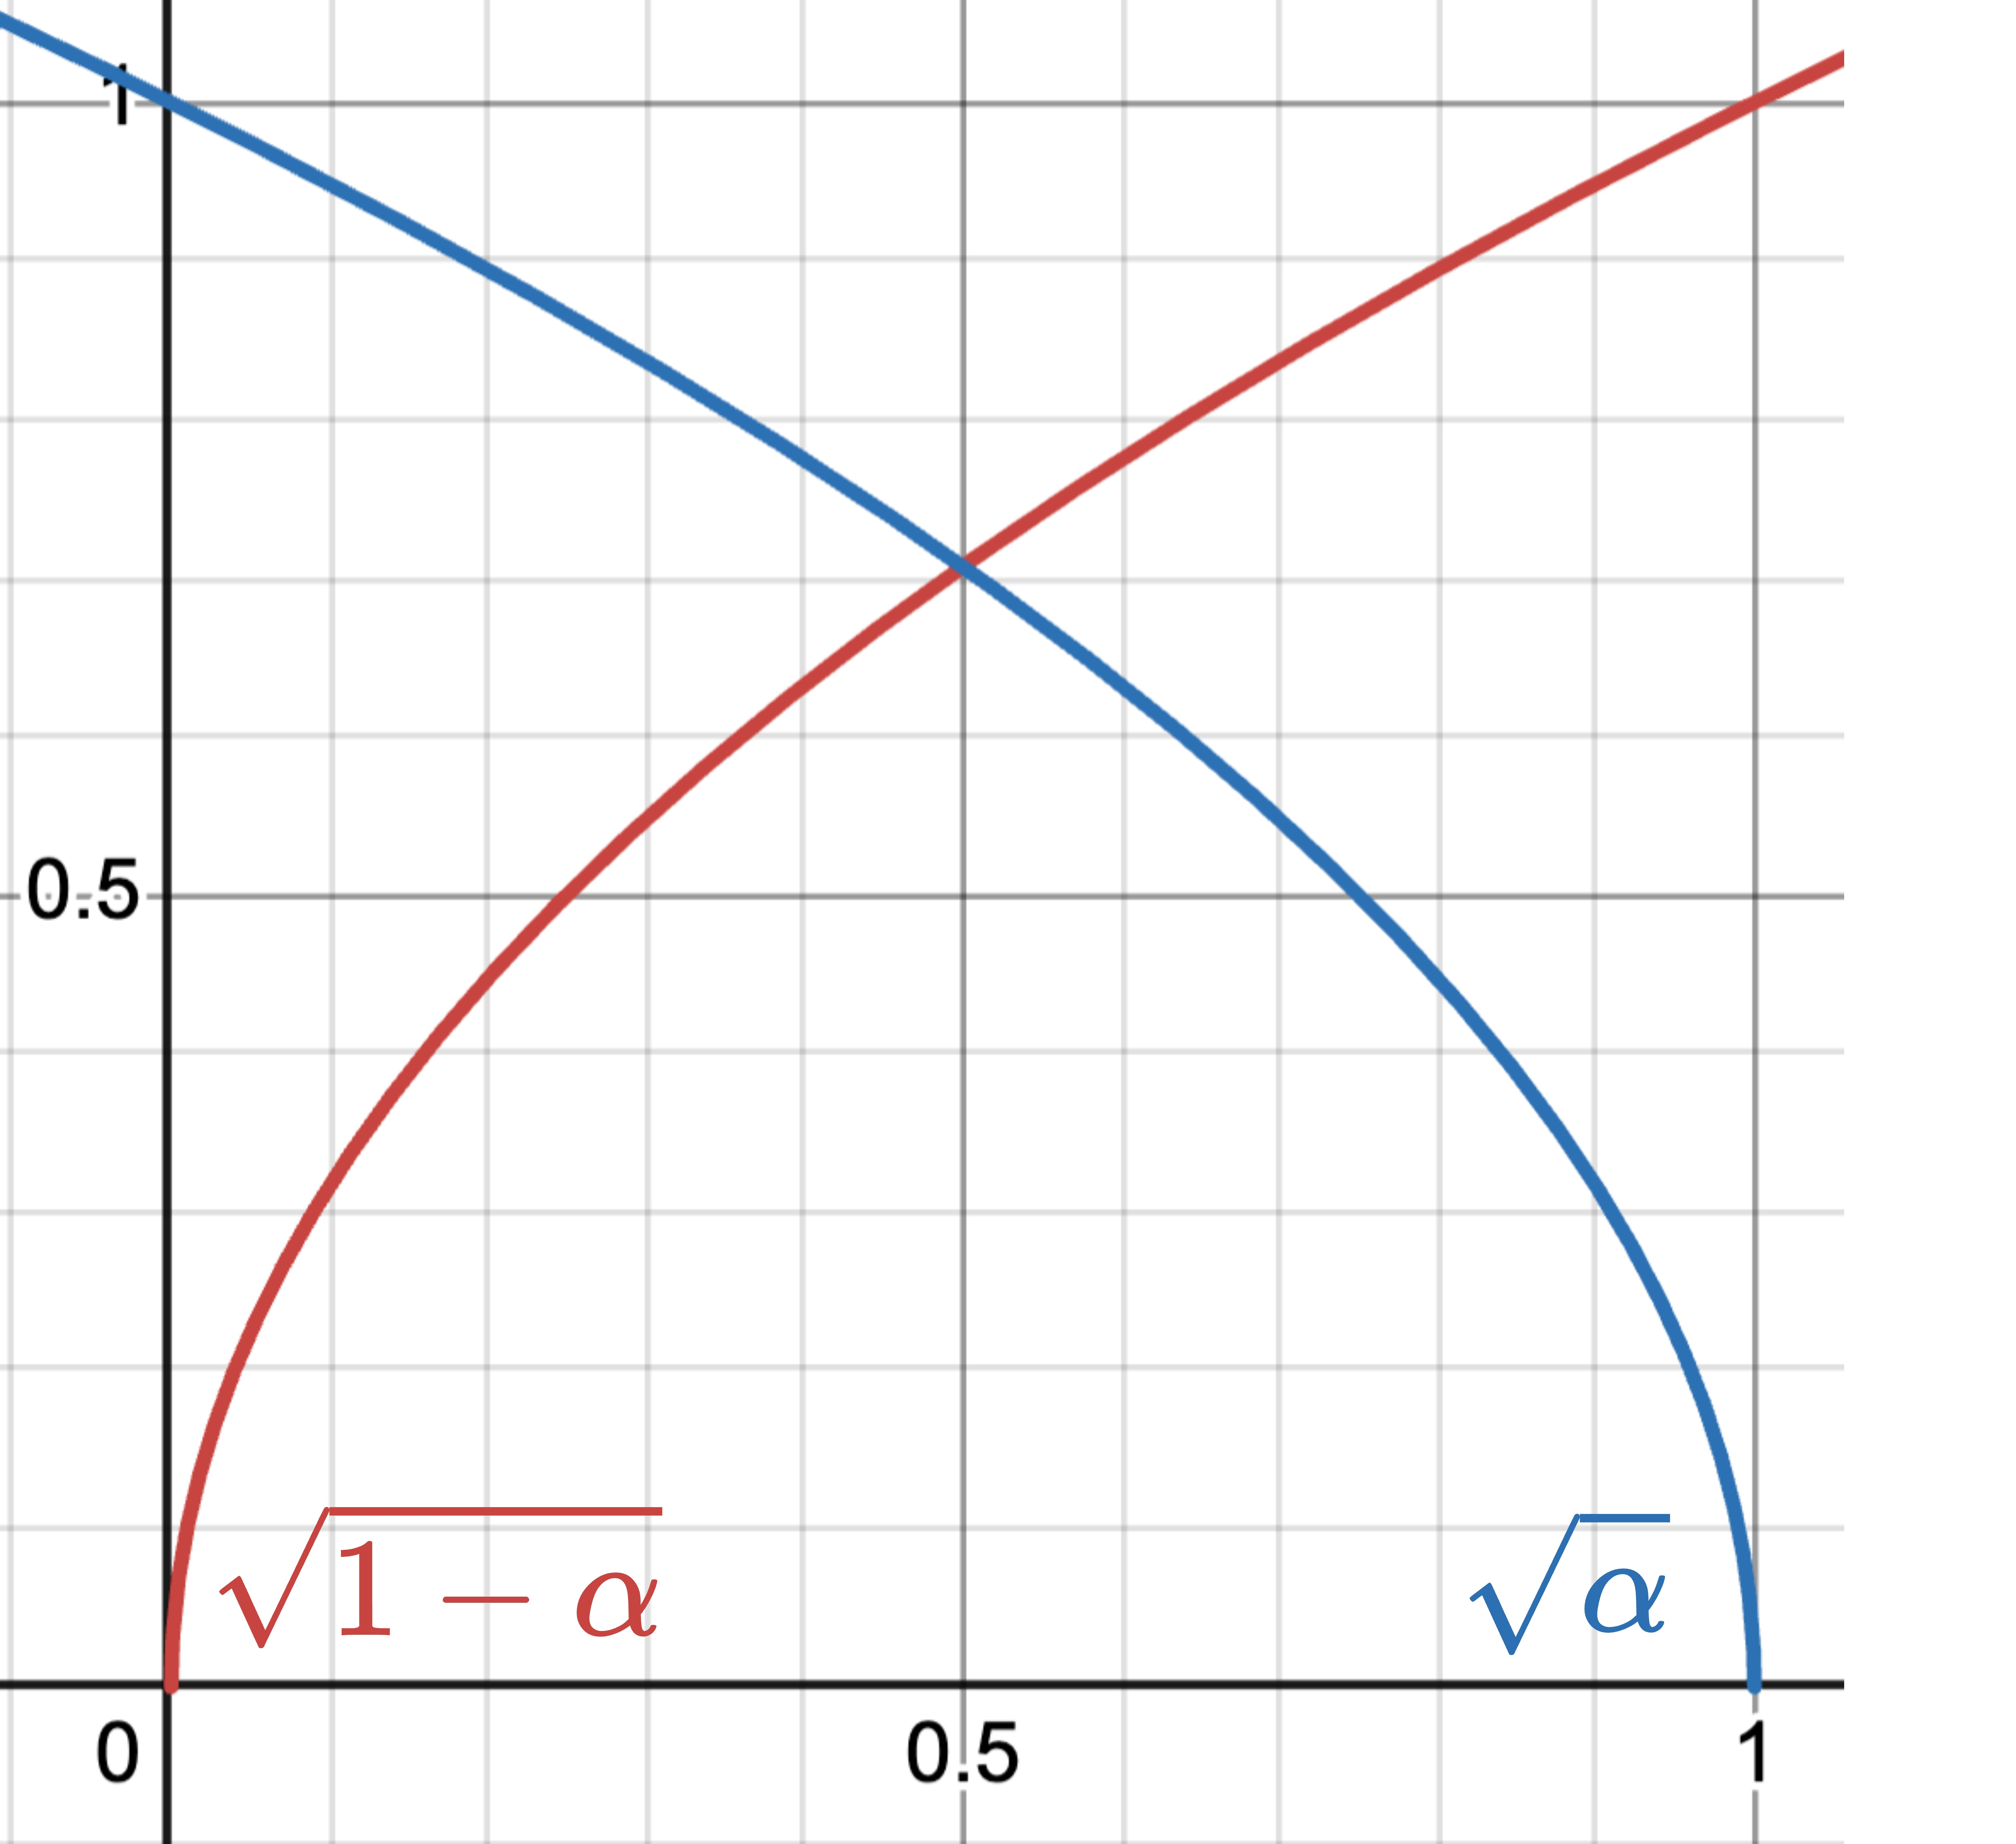
\includegraphics[width=0.5\linewidth]{SquareAlpha}
	\label{fig:wrapfig}
	\caption{Variation of $\sqrt{\alpha}$ and $\sqrt{1 - \alpha}$}
\end{figure}

During the diffusion process, the system aims to gradually reduce the presence of $\bx$ and increase the presence of noise $\epsilon_t$. With $\mathbf{x}_{t} = \sqrt{\alpha_t} \mathbf{x}_{t-1} + \sqrt{1 - \alpha_t} \epsilon_t$, the coefficients $\sqrt{\alpha_t}$ and $\sqrt{1 - \alpha_t}$ control this process as follows:

\begin{itemize}
	\item $\sqrt{\alpha_t}$: Initially has a high value but gradually decreases to reduce the influence of $\bx_t$ in the combined result with noise.
	\item $\sqrt{1 - \alpha_t}$: Initially has a small value but gradually increases at each step, with the goal that eventually the noise dominates and becomes fully noise.
\end{itemize}

Both of these quantities change over time during the diffusion process, determining how much noise is added at each step $t$ and how much of the previous state is retained at each step.

\section{Variation of $\sqrt{\bar{\alpha}}$ and $\sqrt{1 - \bar{\alpha}}$}

$\bar{\alpha}_t = \prod_{i=1}^t \alpha_i$.  $\sqrt{1 - \bar{\alpha}_t} = \sqrt{1 - \prod_{i=1}^t \alpha_i}$. Both $\sqrt{\bar{\alpha}}$ and $\sqrt{1 - \bar{\alpha}}$ play an important role in the training and gesture generation processes. They help control the level of noise added and the gestures generated. It can be observed that $\sqrt{\bar{\alpha}}$ gradually decreases while $\sqrt{1 - \bar{\alpha}}$ increases.

\begin{figure}[h]
	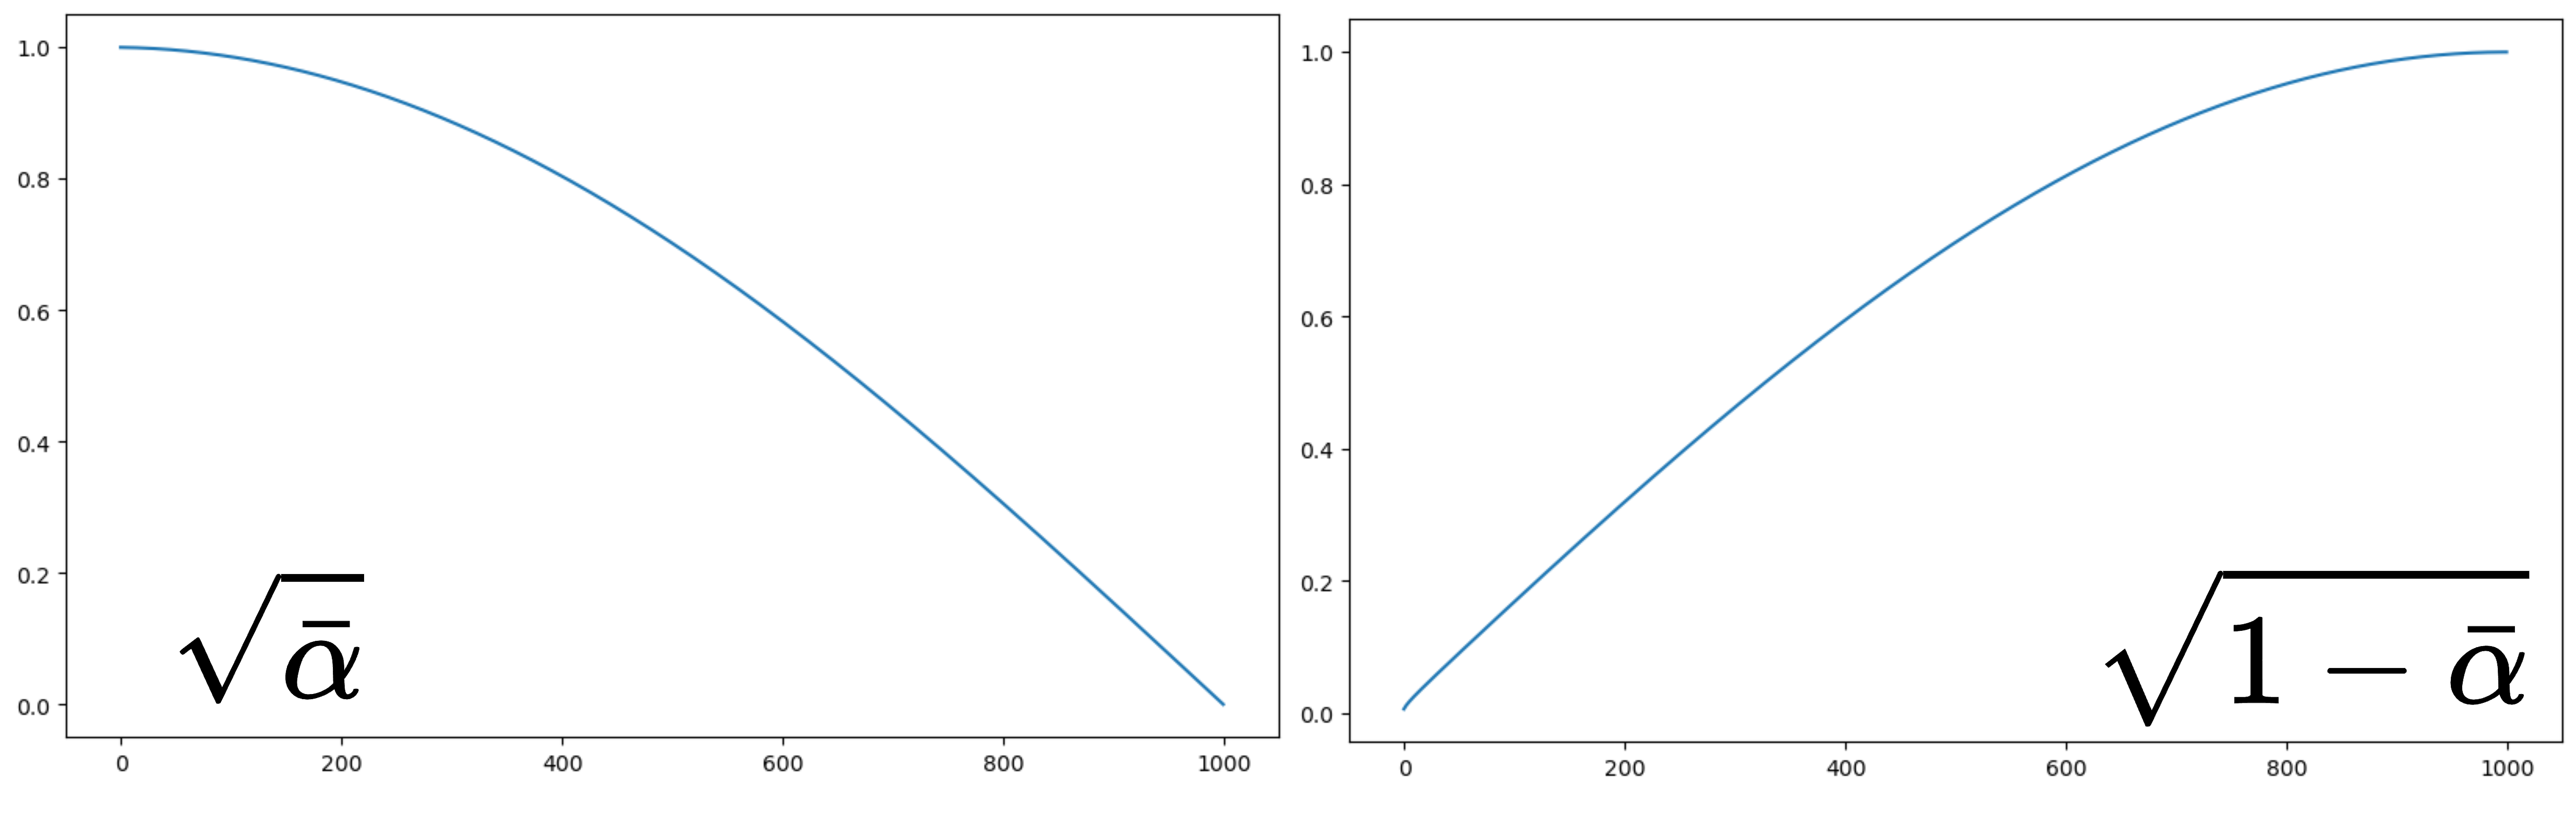
\includegraphics[width=\linewidth]{AlphaCumprod}
	\label{fig:AlphaCumprod}
	\caption{Variation of $\sqrt{\bar{\alpha}}$ and $\sqrt{1 - \bar{\alpha}}$}
\end{figure}

%\section{Comparison of $\epsilon$ objective and $\bx_0$ }

\section{Variation of $\sigma_t$}
\label{appendix:Appendix1:NoiseScale}
\vspace{-10pt}
\begin{figure}[h]
	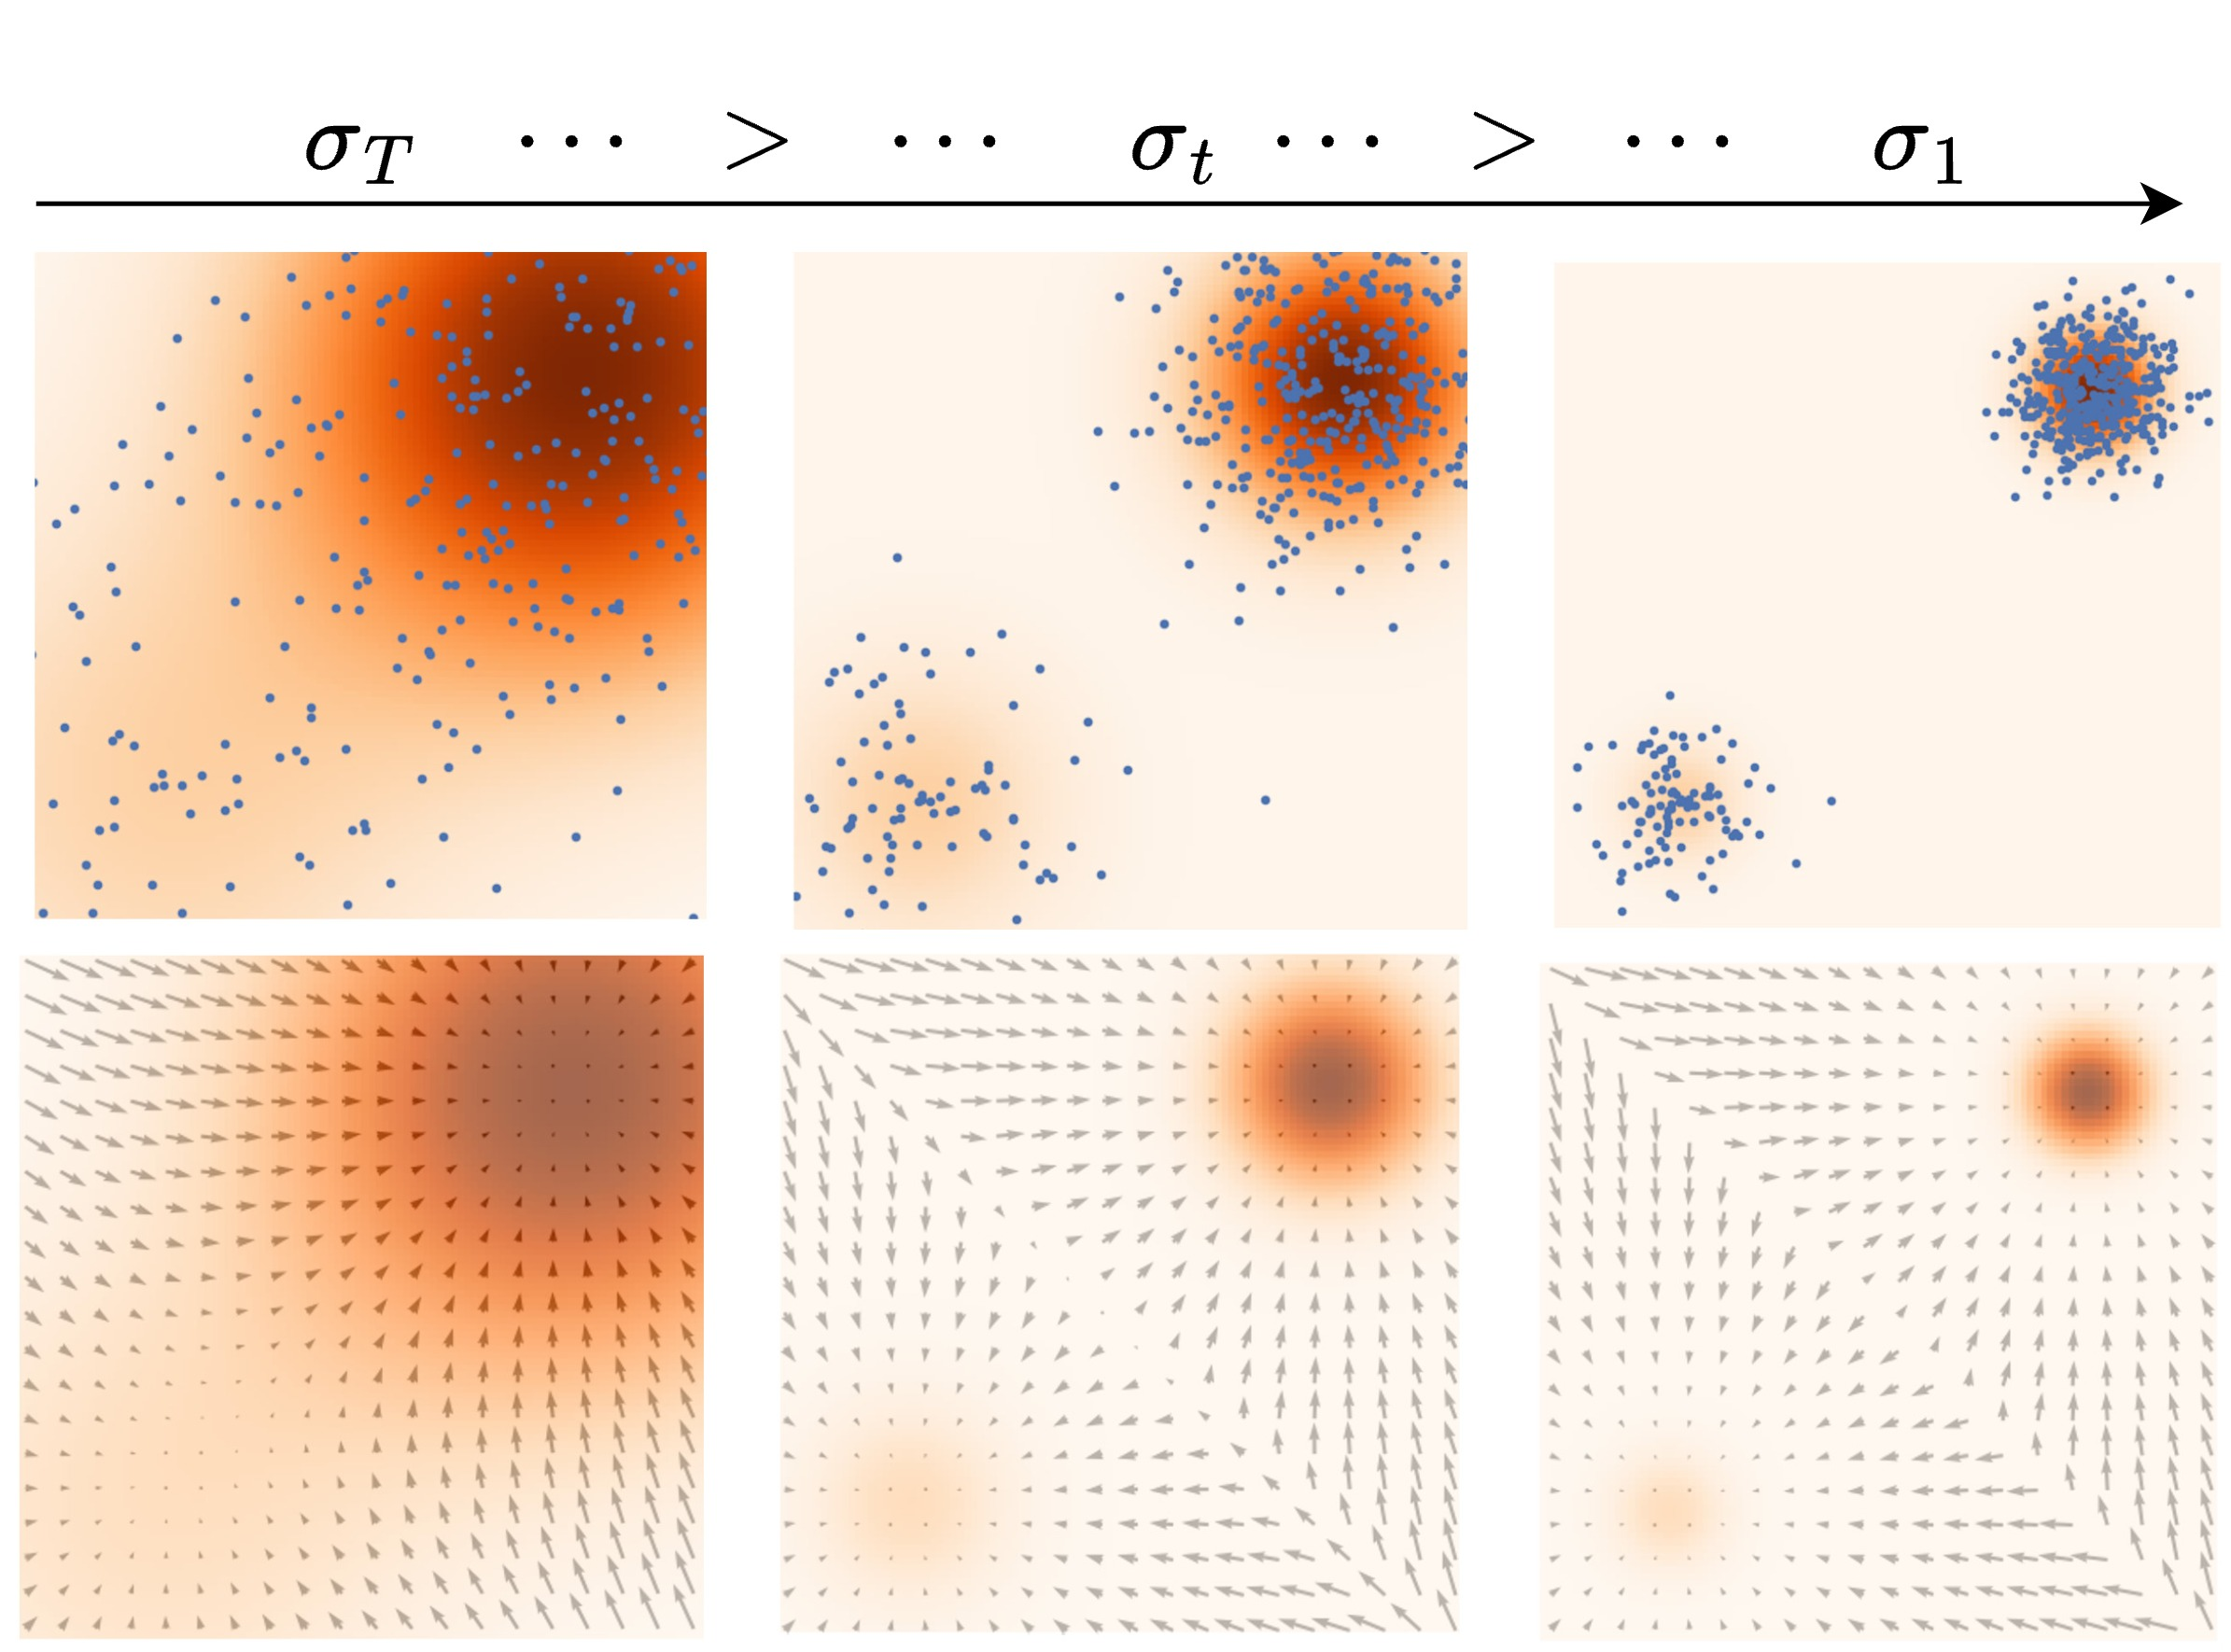
\includegraphics[width=\linewidth]{NoiseScale}
	\label{fig:NoiseScale}
	\caption{Variation of the coefficient $\sigma_t$ during the sampling process}
\end{figure}
\vspace{-10pt}
During the sampling process, the goal of decreasing $\sigma_t$ is to allow the model to navigate toward high-density data regions at each step $t$.

